\section{Detekcja przetworzonych twarzy -- FaceForensics++}
Artykuł `FaceForensics++' rozpatruje szereg istotnych zagadnień w dziedzinie detekcji manipulacji twarzy~\cite{rossler2019faceforensics++}.
Przede wszystkim, przedstawia zautomatyzowany benchmark do wykrywania manipulacji twarzy w przypadku losowej kompresji, co umożliwia standaryzowane porównanie różnych metod detekcji.
Benchmark ten obejmuje także bazową ocenę przeprowadzaną przez ludzi, co umożliwia porównanie skuteczności automatycznych systemów detekcji do wyników uzyskanych przez ekspertów.

\begin{figure}[h]
    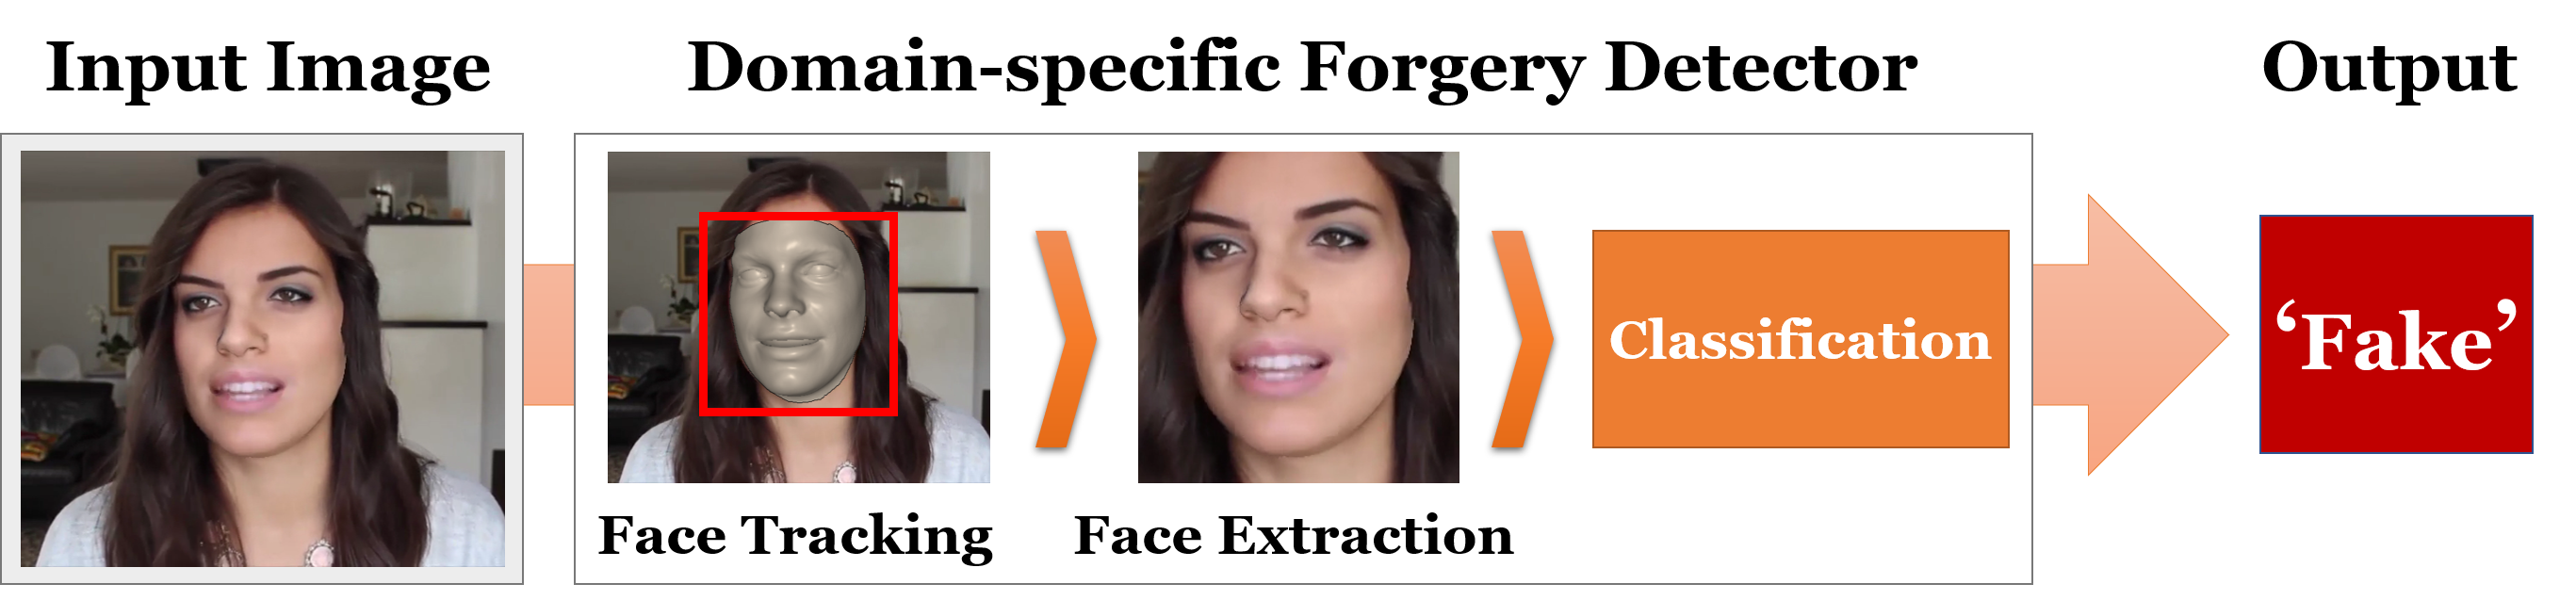
\includegraphics[width=0.9\linewidth]{img/FF++detection_pipeline}
    \caption{ Wizualne przedastwanie kroków działania FaceForensics++.
    Obraz wejściowy jest przetwarzany przez metodę śledzenia twarzy; informacje są wykorzystywane do wyodrębnienia obszaru obrazu pokrytego twarzą. Następnie ten obszar jest podawany na wejście nauczonej sieci klasyfikacyjnej, która generuje predykcję.
    Źródło~\cite{rossler2019faceforensics++}:}
    \label{img:FFPileline}
\end{figure}

Kolejnym ważnym wkładem naszego artykułu jest stworzenie innowacyjnego i obszernego zbioru danych do nauki.
Zbiór ten zawiera ponad 1,8 miliona obrazów pochodzących z 1000 filmów, które przedstawiają manipulowane obrazy twarzy.
Co więcej, dla każdego manipulowanego obrazu posiadamy również oryginalne obrazy stanowiące dane referencyjne.
Dzięki temu zbiór ten umożliwia nadzorowane uczenie się systemów detekcji, co pozwala na poprawę ich skuteczności.

Nasz artykuł obejmuje również obszerną ocenę najnowocześniejszych detektorów fałszerstw, zarówno opartych na metodach manualnych, jak i na uczeniu maszynowym.
Przeprowadziliśmy tę ocenę w różnych scenariuszach, co pozwoliło nam zrozumieć i porównać skuteczność tych detektorów w różnych kontekstach.
Dzięki temu dostarczamy wglądu w najlepsze obecnie dostępne metody detekcji manipulacji twarzy.

Ostatecznie, artykuł przedstawia najnowocześniejszą metodę detekcji fałszerstw, stworzoną specjalnie do manipulacji twarzy.
Ta metoda wykorzystuje najnowsze osiągnięcia w dziedzinie detekcji manipulacji obrazów, aby zapewnić wysoką skuteczność w wykrywaniu manipulacji twarzy.

Wszystkie te wkłady mają na celu rozwinięcie dziedziny detekcji manipulacji twarzy i dostarczenie narzędzi oraz wiedzy, które przyczynią się do poprawy bezpieczeństwa w obszarze rozpoznawania twarzy i zwalczania manipulacji obrazów.

W obecnych metodach manipulacji obrazem twarzy, które są uważane za najlepsze w swojej kategorii, demonstrujemy, że można je wykryć za pomocą szkoleniowych detektorów fałszerstw.
Szczególnie zachęcające jest to, że trudny przypadek niskiej jakości wideo może być rozwiązany za pomocą podejścia opartego na uczeniu maszynowym, gdzie ludzie i ręcznie opracowane cechy napotykają trudności.

Autorzy FaceForresic++ stworzyli standaryzowany benchmark dla dalszych prac.
Wszystkie dane obrazowe, szkoleniowe modele oraz benchmark są publicznie dostępne i są już wykorzystywane przez innych badaczy.
W szczególności `zero-shot learning' ma duże znaczenie, gdyż w miarę pojawiania się nowych metod manipulacji, konieczne jest opracowanie metod umożliwiających wykrywanie fałszerstw przy niewielkim lub żadnym dostępnym zbiorze danych treningowych.


\section{Lokalizowanie anormalnych cech obrazów -- ManTra-Net}

\begin{figure}[h]
    \centering
    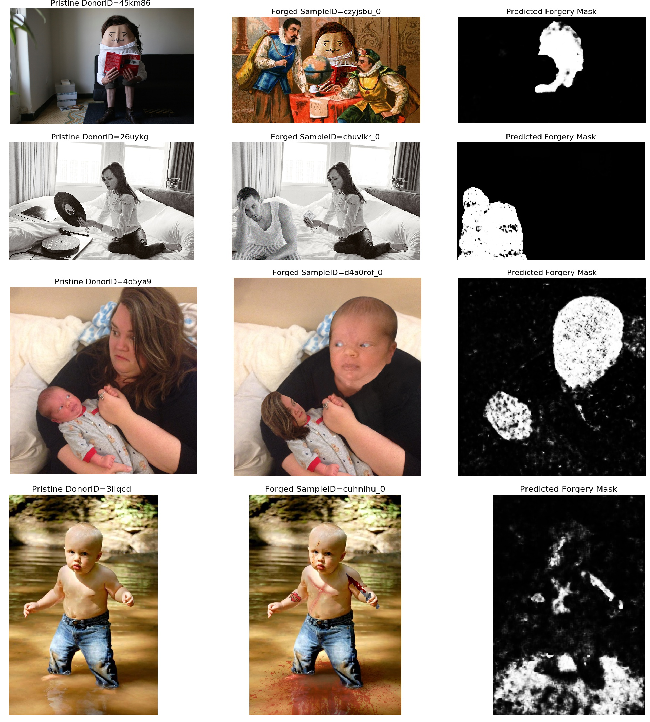
\includegraphics[width=0.7\linewidth]{img/mantra-net-example}
    \caption{Obraz iluctrujacy działanie MantraNet. Pierwsza kolumna od lewj pokazuje niezmieniony obraz.
    Kolejna kolumna pokazuje zmieniony obraz będoący wejsćiem do sieci. Piewsza kolumna od prawej to wyjście z sieci.
    Wyjściem z sieci jest obraz w odcieniach szarosci, gdzie kolor czarny oznacza brak zmiany a kolor biały oznacza że zmiana jest pewna.
    Źródło~\cite{ManTraNet}:}
    \label{fig:mantra-net}
\end{figure}

ManTra-Net to sieć neuronowa, która wykonuje zarówno detekcję, jak i lokalizację manipulacji bez dodatkowego przetwarzania wstępnego i poprzedzającego~\cite{ManTraNet}.
Jest to sieć w pełni konwolucyjna, która obsługuje obrazy o dowolnych rozmiarach oraz wiele znanych rodzajów fałszerstw, takich jak przycinanie, kopiowanie, usuwanie, poprawianie, a nawet nieznane typy manipulacji.
Działanie modelu pokazano na obrazie~\ref{fig:mantra-net}.

Artykuł ma trzy istotne wkłady.
Po pierwsze, pokazuje zbieżną metodę uczenia bez nadzoru, które pozwala na naukę wykrywania śladów manipulacji obrazem poprzez klasyfikację 385 rodzajów manipulacji obrazem.
Po drugie, formułujemy problem lokalizacji fałszerstw jako problem lokalnego wykrywania anomalii, wykorzystując cechę Z-score, która pozwala na wykrywanie lokalnych anomalii, oraz proponują nowatorskie rozwiązanie z wykorzystaniem długotrwałej pamięci krótkoterminowej(LSTM) w celu oceny lokalnych anomalii.
Na koniec przeprowadzono eksperymenty różnicowe, aby systematycznie optymalizować projekt sieci.
Wyniki eksperymentalne dowodzą ogólnego zastosowania, odporności i przewagi ManTra-Net, nie tylko w pojedynczych typach manipulacji/fałszerstw, ale także w ich skomplikowanych kombinacjach.

ManTra-Net to potężne narzędzie, które umożliwia wykrywanie i lokalizację różnych rodzajów manipulacji obrazów.
Zdolność do obsługi obrazów o różnych rozmiarach i różnych typów manipulacji czyni go wszechstronnym i przydatnym w różnych scenariuszach.
Wyniki eksperymentalne potwierdzają skuteczność i niezawodność tej technologii, co stanowi istotny wkład w dziedzinie analizy manipulacji obrazów.


\section{Detekcja przetworzonych twarzy –- MeasoNet}

MeasoNet to model do automatycznego i efektywnego wykrywania manipulacji twarzy w wideo, ze szczególnym uwzględnieniem dwóch niedawno stosowanych technik generowania sfałszowanych wideo: Deepfake i Face2Face~\cite{mesoNet}.
Tradycyjne techniki kryminalistyki obrazu zazwyczaj nie są odpowiednie dla wideo ze względu na kompresję, która silnie degraduje dane.
Dlatego w niniejszej publikacji stosuje się podejście oparte o dwie sieci o niewielkiej liczbie warstw, aby skupić się na właściwościach obrazów.
Ocena tych szybkich sieci przeprowadzana jest zarówno na istniejącym zbiorze danych, jak i na zbiorze danych stworzonym z wideo dostępnych online.
Twórcy wykorzystali test stworzony przez zespół FaceForenzic++.
Testy wykazują bardzo wysoką skuteczność wykrywania, wynoszącą ponad 98\% dla Deepfake i 95\% dla Face2Face.


W tej sekcji przedstawiane są kilka skutecznych podejść do radzenia sobie zarówno z problemem Deepfake, jak i Face2Face.
Okazało się, że te dwa problemy mogą być skutecznie rozwiązane przy użyciu pojedynczej sieci.
Jednak dzięki podobnej naturze fałszerstw, identyczne struktury sieciowe dla obu problemów mogą dawać dobre rezultaty.

Proponuje się wykrywanie sfałszowanych wideo twarzy poprzez umieszczenie metody na mezoskopowym poziomie analizy.
Rzeczywiście, mikroskopowe analizy oparte na szumach obrazu nie mogą być zastosowane w kontekście skompresowanego wideo, gdzie szum obrazu jest znacznie zdegradowany.
Podobnie na wyższym poziomie semantycznym ludzkie oko ma trudności w rozróżnianiu sfałszowanych obrazów, zwłaszcza gdy obraz przedstawia ludzką twarz.
Dlatego proponuje się przyjęcie pośredniego podejścia, polegającego na wykorzystaniu głębokiej sieci neuronowej o niewielkiej liczbie warstw.

Dwie następujące architektury osiągnęły najlepsze wyniki klasyfikacji spośród wszystkich testów, przy niskim poziomie reprezentacji i zadziwiająco niskiej liczbie parametrów.
Opierają się one na dobrze działających sieciach do klasyfikacji obrazów [14, 23], które na przemian wykorzystują warstwy splotowe i pooling do ekstrakcji cech, oraz gęstą sieć do klasyfikacji.


\section{Analzia poziomu błędów (ang. \textit{Error level analysis})}

Error Level Analysis (ELA) to metoda analizy obrazów, która służy do wykrywania zmian i manipulacji w cyfrowych obrazach.
Polega na porównywaniu poziomów kompresji w różnych obszarach obrazu, aby zidentyfikować obszary o potencjalnych zmianach.

Proces ELA polega na kompresowaniu oryginalnego obrazu cyfrowego z użyciem określonego algorytmu kompresji, na przykład JPEG, a następnie porównaniu otrzymanego obrazu skompresowanego z oryginalnym obrazem.
Różnice między tymi dwoma wersjami obrazu wskazują obszary, które mogły ulec manipulacji lub edycji.

Opis procesu ELA:

Konwersja do formatu JPEG: Oryginalny obraz jest konwertowany na format JPEG z wybranym poziomem kompresji.
Kompresja JPEG jest stratnym algorytmem kompresji, który usuwa niektóre szczegóły obrazu i wprowadza pewne artefakty.

Porównanie poziomów kompresji: Porównuje się otrzymany skompresowany obraz z oryginalnym obrazem, piksel po pikselu.
Różnice w poziomach kompresji wskazują obszary, które mogą ulec manipulacji.

Wygenerowanie mapy błędów: Na podstawie różnic w poziomach kompresji generowana jest tzw.
mapa błędów, która wizualizuje obszary o potencjalnych zmianach.
Obszary o wysokim stopniu zmian mają jasne lub intensywne kolory, podczas gdy obszary bez zmian są bardziej jednolite.

Interpretacja wyników: Analiza mapy błędów pozwala zidentyfikować obszary, które mogły ulec manipulacji.
Na przykład, obszary o wysokim stopniu zmian mogą wskazywać na dodanie, usunięcie lub zmianę pewnych elementów w obrazie.

ELA ma swoje ograniczenia i nie jest narzędziem idealnym.
Wyniki analizy ELA mogą być podatne na pewne błędy interpretacyjne, zwłaszcza w przypadku obrazów o różnych stopniach detali, tekstur i złożoności.
Ponadto, analiza ELA może wykrywać zmiany w kompresji, ale nie jest w stanie jednoznacznie ustalić, jakie dokładnie zmiany zostały wprowadzone w obrazie.

Mimo tych ograniczeń analiza poziomu błędów jest jednym z narzędzi stosowanych w cyfrowej obróbce zdjęć i badaniu autentyczności obrazów, pomagając w identyfikacji potencjalnych manipulacji i zmian w obrazach cyfrowych.